cd \documentclass{standalone}
\usepackage{tikz,pgfplots,calc}
\usetikzlibrary{positioning,calc}
\usetikzlibrary{arrows}
\usepackage{tkz-euclide}
\usetkzobj{all}

\renewcommand{\familydefault}{\sfdefault}
\begin{document}
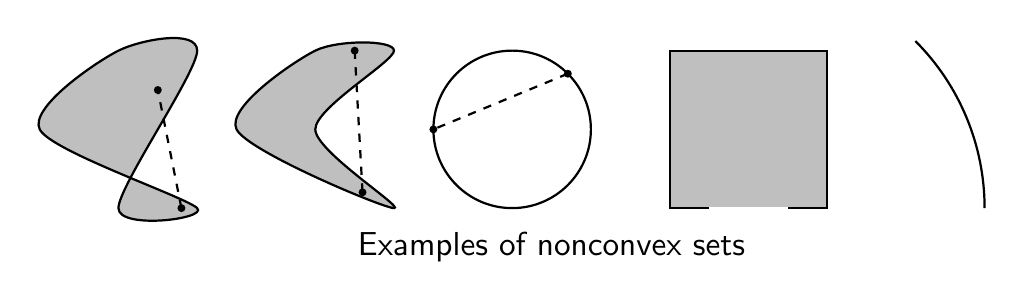
\begin{tikzpicture}[>=stealth', thick]

\begin{scope}
    \draw [fill = gray!50] plot [smooth cycle] coordinates {(0,0) (1,1) (2,1) (1,-1) (2,-1)};

    \draw [fill] (1.5, .5) circle (1pt);
    \draw [fill] (1.8, -1) circle (1pt);
    \draw [dashed] (1.8, -1) -- (1.5, .5);
\end{scope}

\begin{scope}[xshift = 2.5cm]
    \draw [fill = gray!50] plot [smooth cycle] coordinates {(0,0) (1,1) (2,1) (1,0) (2,-1)};
    \draw [fill] (1.5, 1) circle (1pt);
    \draw [fill] (1.6, -.8) circle (1pt);
    \draw [dashed] (1.5, 1) -- (1.6, -.8);
\end{scope}

\begin{scope}[xshift = 6cm]
    \draw  (0, 0) circle (1cm);
    \draw [fill] ({sqrt(2)/2}, {sqrt(2)/2}) circle (1pt);
    \draw [fill] (-1, 0) circle (1pt);

    \draw [dashed] (({sqrt(2)/2}, {sqrt(2)/2}) -- (-1, 0);
\end{scope}

\begin{scope}[xshift = 9cm]
    
    \draw [black] (3, -1) arc(0:45:3cm); %now ok
    % \draw [] plot [smooth] coordinates {(0,0) (1,1) (2, 1)};
    \draw [fill = gray!50, draw = white] (-1, -1) rectangle (1, 1);
    \draw (-.5, -1) -- (-1, -1) -- (-1, 1) -- (1, 1) -- (1, -1) -- (.5, -1);
\end{scope}
\node [scale = 1.2] at (6.5, -1.5) {Examples of nonconvex sets};
\end{tikzpicture}
\end{document}